\documentclass[journal,onecolumn]{IEEEtran}
%\usepackage[left=2.2cm,right=2.2cm,top=2.5cm,bottom=2.5cm]{geometry}
\usepackage[utf8]{inputenc}
\usepackage{minted}
\usepackage{booktabs}
\usepackage{commath}
\usepackage{float}
\usepackage{mathtools}
\usepackage{color}
\usepackage{amsthm}
\usepackage{parskip}


\usepackage[binary-units=true]{siunitx}

\newcommand{\py}[1]{\mintinline{python}{#1}}

\title{Artificial Intelligence (\texttt{LINGI2261}) \\ Assignment 3 --- Group 13}
\author{Martin Braquet, Gilles Peiffer}
\date{November 27, 2019}

\begin{document}

\maketitle

\section{Alpha-Beta Search}
Figure~\ref{fig:minimax} can be obtained by applying the minimax algorithm to the tree given in the statement.
\subsection{MiniMax Algorithm}
\begin{figure}[H]
 \centering
 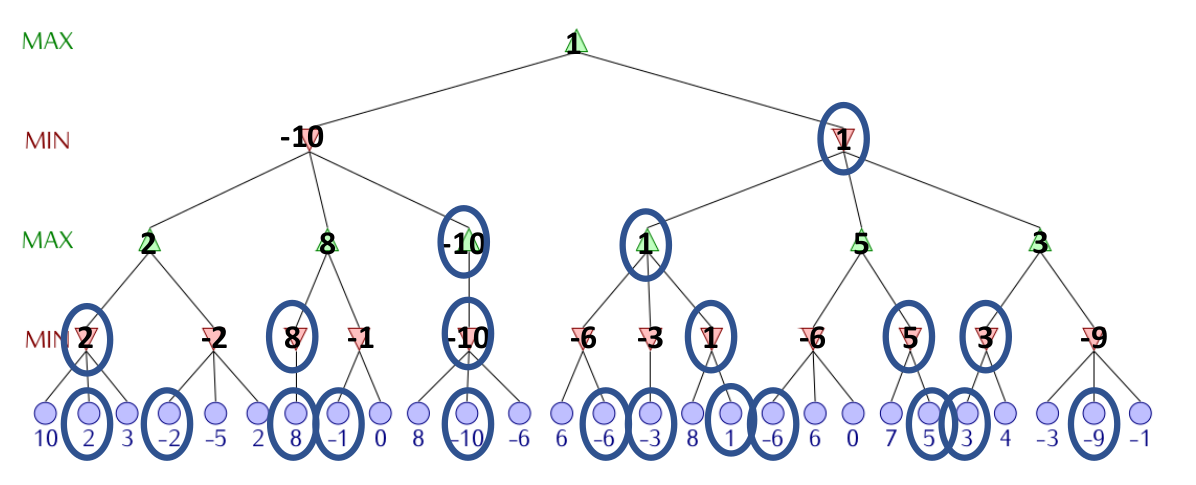
\includegraphics[width=\textwidth]{img/MiniMax.png}
 \caption{Minimax algorithm}
 \label{fig:minimax}
\end{figure}
One notices that nodes in the ``MAX'' nodes simply take on the highest value among their child nodes, whereas ``MIN'' nodes take on the lowest value among their child nodes.

\subsection{Alpha-Beta Algorithm (Left To Right)}
Using a technique called ``Alpha-Beta pruning'', the number of nodes which have to be explored can be reduced (though it stays exponential in the worst case).
This is shown in Figures~\ref{fig:alphabeta} and \ref{fig:alphabeta_reverse}.
\begin{figure}[H]
 \centering
 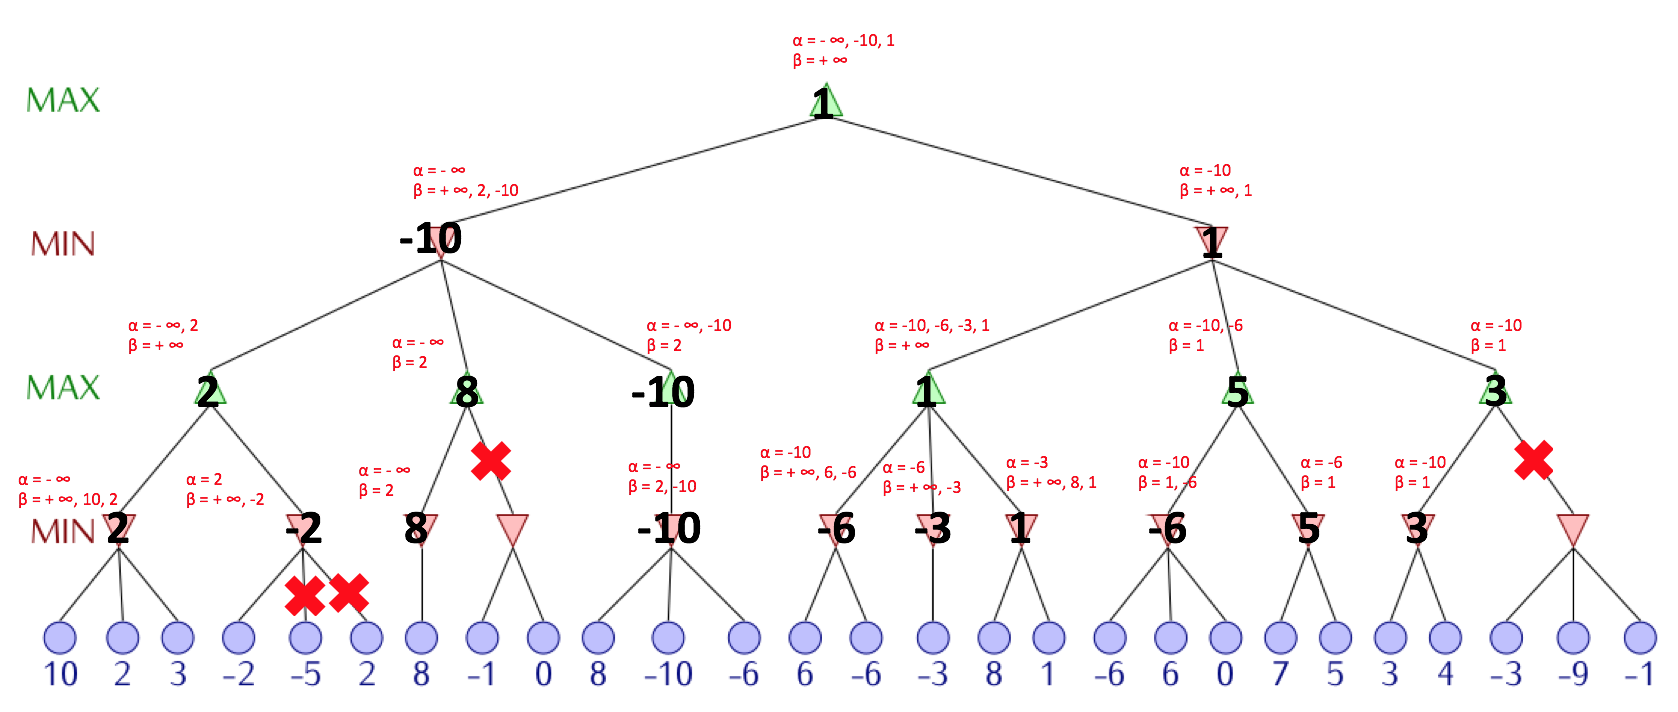
\includegraphics[width=\textwidth]{img/Alphabeta.png}
 \caption{Alpha-Beta algorithm (left to right)}
 \label{fig:alphabeta}
\end{figure}
Every red cross denotes a pruning operation.
For example, the two leftmost prunings are possible because no matter what values \(x\) and \(y\), they give, their parent node is going to take on value \(\min\{-2, x, y\} \le -2 < 2\), which is the value which is going to be conserved when moving up to the ``MAX'' node on the row above.
The values of \(\alpha\) and \(\beta\) are used to keep track of when a subtree can be pruned.

\subsection{Alpha-Beta Algorithm (Right To Left)}
\begin{figure}[H]
 \centering
 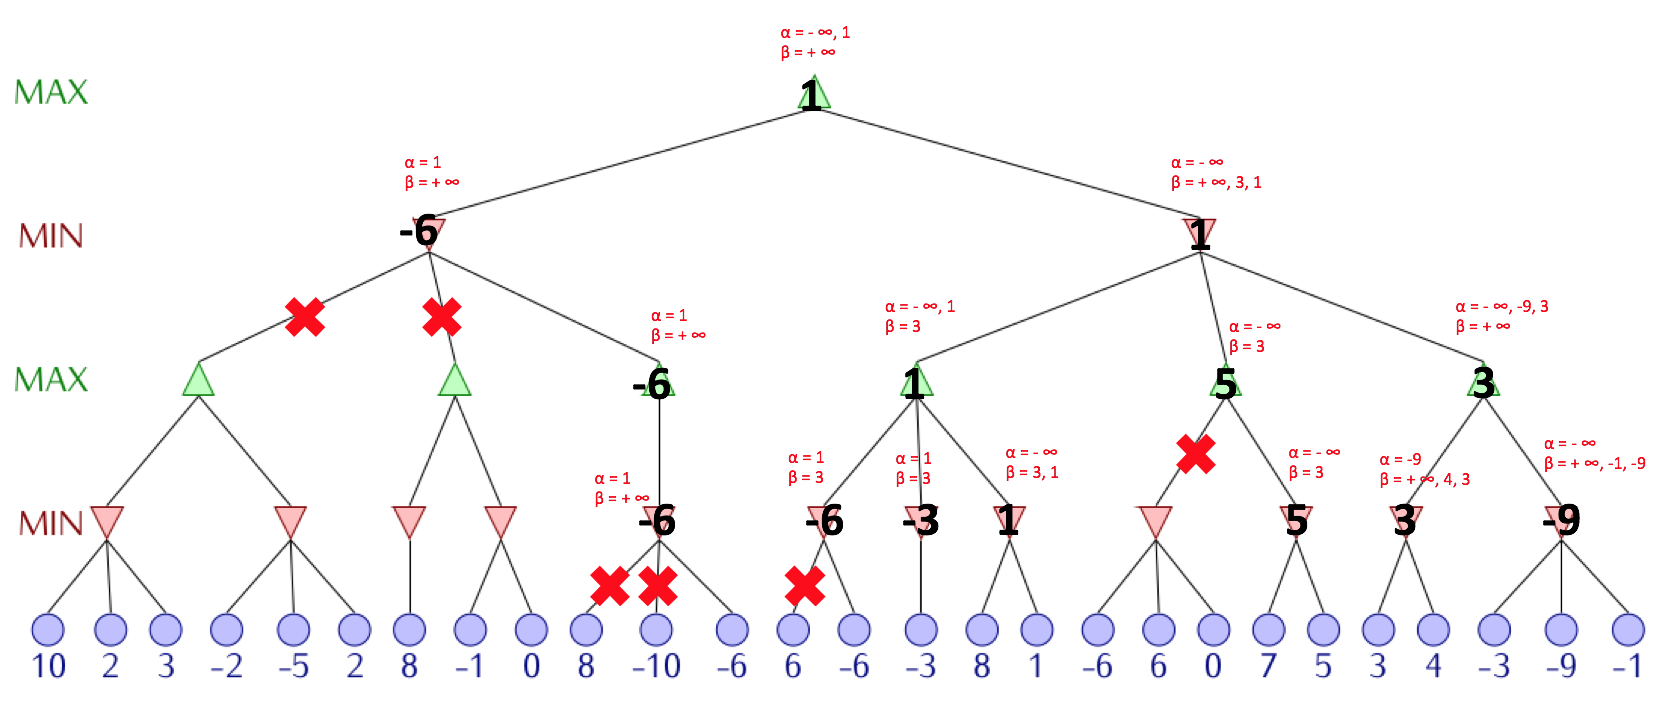
\includegraphics[width=\textwidth]{img/Alphabeta_reverse.png}
 \caption{Alpha-Beta algorithm (right to left)}
 \label{fig:alphabeta_reverse}
\end{figure}


\subsection{Alpha-Beta Algorithm (Ordered)}
Using this pruning algorithm, it is possible to find an ordering of the nodes which, when used to determine which nodes are explored first, minimizes the amount of nodes that need to be explored.
This optimal tree is shown in Figure~\ref{fig:alphabeta_ordered}, assuming a left-to-right exploration.
To obtain this tree, one needs to order nodes in ascending order on MAX levels and in descending order on MIN levels.
\begin{figure}[H]
 \centering
 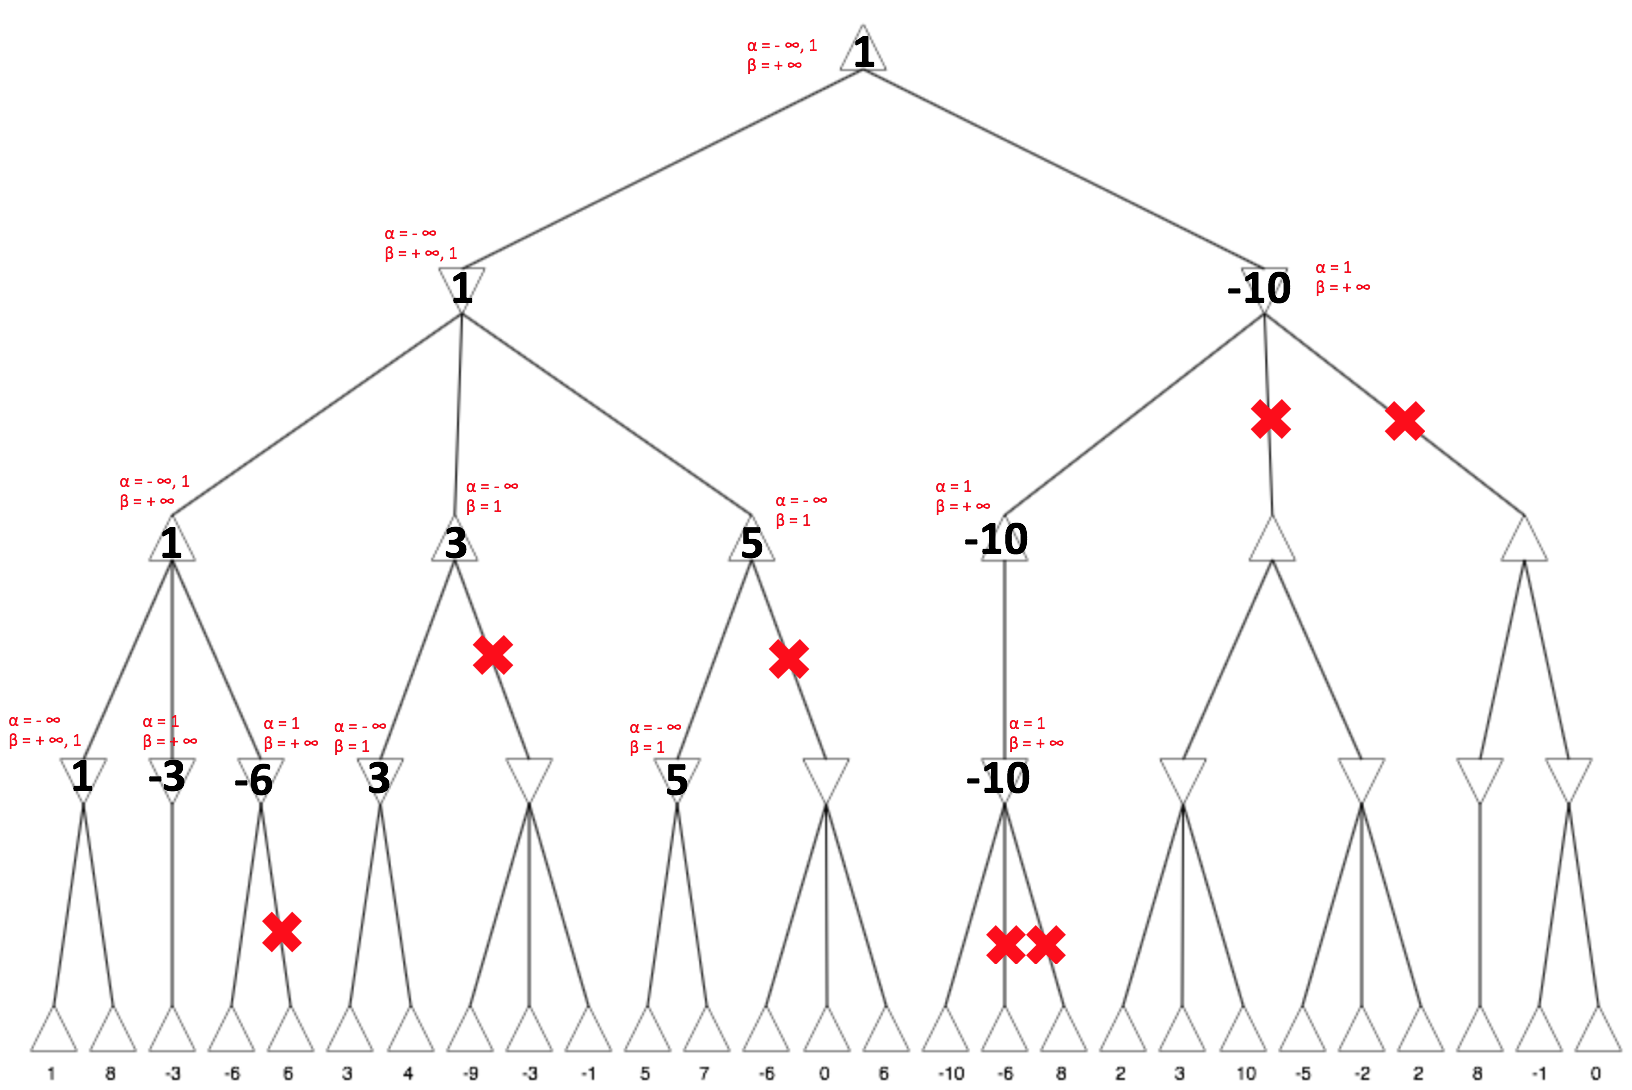
\includegraphics[width=\textwidth]{img/Alphabeta_ordered.png}
 \caption{Alpha-Beta algorithm}
 \label{fig:alphabeta_ordered}
\end{figure}

\subsection{Alpha-Beta For More Than Two Players}
For games with more than two players, each node is associated with a tuple giving the value of each player for that state.

Tree pruning is possible if there is an upper bound on the sum of all components of this tuple, and if there is a lower bound on the values of each component.
We define the sum $S$ as the global upper bound on the sum of all components of the \(N\)-tuple, and all components are assumed to be nonnegative. 

The conditions \py{v <= alpha} and \py{v >= beta} are now given by \py{Best[Player] >= Bound} where the bound equals the sum $S$ minus the last best node of the upper layer.
Indeed, let us take a player 1 from the upper layer which is ensured to get a value of at least $x$ for his layer: $(\ge x, \dots, \dots)$. Then, if player 2 from the lower layer unveils a child with more than $S - x$ for its own value, it will result in a score of $(\le x, \ge S - x, \dots)$. Thus, all the remaining children can be dropped since player 1 knows that these children will be chosen by player 2 only if the value of player 1 is less than $x$. \cite{multiplayer}

\begin{figure}[H]
 \centering
 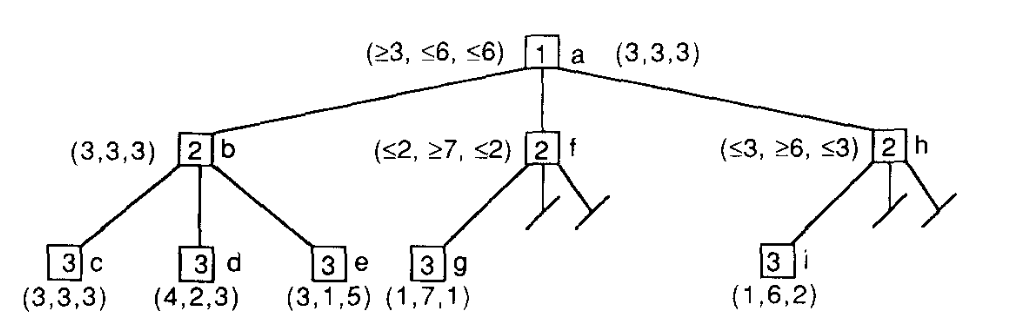
\includegraphics[width=0.7\textwidth]{img/multiplayer.png}
 \caption{Shallow pruning in three-player game tree \cite{multiplayer}}
 \label{fig:multiplayer}
\end{figure}


\section{Squadro}

\subsection{Comparison Of Two Evaluation Functions}
One would expect that the new evaluation will work better since it takes into account the opponent, and will thus try to prevent them from winning, for example, by killing their pawns.
The old agent is not able to deliberately kill the opponent, consequently decreasing its chances of winning.

However, the yellow player still always wins in the four possible starting configurations because it begins with the best pawns at the center, progressing by steps of three.
The yellow player rapidly puts these pawns on the other side, which then form a barrier for the opponent's progress.
Thus, when the depth of the minimax algorithm is not sufficient, the new basic agent is not good enough to overcome the yellow player's innate advantage.

\subsection{Cut-Off Function}
The \emph{depth} in the \py{minimax.py} implementation is the number of steps along the path from the root node to a node in the layer where we stop the tree search and evaluate the node.

When the depth increases, the new basic agent is able to win even when playing as the red player because it can now predict and find a counter-attack against the yellow barrier.
The new basic agent wins for all starting configurations when the depth is higher than six.

Since the Squadro contest has a time limit, one needs to select the time allowed for each move.
There exist different methods to choose the maximum time allowed for each search, but an interesting option is to decrease the allotted time throughout the game in order to prevent exceeding the limit.
Indeed, one can split the time for each move $t_\textnormal{move}$ according to the next formula:
\[
    t_\textnormal{move} = 
    \left\{
    \begin{array}{ll}
      0.2 \: t_\textnormal{left}^2, & \mathrm{if}\quad t_\textnormal{left}\leq \min\{\SI{100}{s}, t_\textnormal{total}/3\}, \\
      20, & \mathrm{otherwise.} \\
    \end{array} 
    \right.
\]
where $t_\textnormal{left}$ is the remaining amount of time for the considered player and \(t_\textnormal{total}\) is the initial time limit.
One can notice that the allowed time goes to zero as the remaining time drops, as expected.

Using iterative deepening is a good choice to stop the algorithm during its search.
Iterative deepening depth-first search is a search method which iteratively performs a depth-limited depth-first search using the minimax algorithm, starting from a limit depth of one, up to some predefined value.
By recording the optimal path at each depth, the moves can be ordered in such a way as to minimize the total search time, coompensating for the (asymptotically negligible) cost of searching with lower depth limits.

The depth is chosen so that the algorithm gives good results, for instance eight.
However, when time runs out, the program returns the move selected by the deepest completed search.

The cut-off function, which reflects the moment when we need to stop the search, is activated when one of the following three conditions is true:
\begin{enumerate}
 \item \py{depth > self.current_depth}: the depth of the analyzed node is higher than the maximum depth,
 \item \py{state.game_over_check()}: the game is over,
 \item \py{time() - self.start_time > self.max_time}: the time elapsed during this search has exceeded the maximum allowed period for this search.
\end{enumerate}

\subsection{Evaluation Function}
In the figure presented in the instructions, the yellow basic agent will move its pawn number 3 since it will lead to the highest value of its evaluation function: the sum over all pawns of each's advancement.
However, it is clear that this is not the best possible move, since moving pawn number 4 would make it win the game.
A stronger heuristic thus has to take into account that a player wins if only four of their pawns return to their initial position.
In practice, we reduce this progress evaluation to only the four most advanced pawns, bringing a more cogent representation of the state.

The weak points of the evaluation function of the basic agents are
\begin{itemize}
	\item The first basic agent always tries to maximize its own total advancement, meaning that it does not take into account changes to the total advancement of the opponent.
	The second basic agent solves this by trying to maximize the difference between the total advancements.
	\item Both basic agents fail to recognize a potential game-winning move, which is solved in the smart agent by adding the requirement on the number of pawns which need to return to their initial position to win the game.
\end{itemize}

In addition to the sum of each pawn’s advancements, the following features are detailed below: the smart agent looks at
\begin{itemize}
 \item the total advancement of both players; and
 \item the number of pawns which have reached their initial position again.
\end{itemize}

The improved evaluation function thus takes into account these two features.
\begin{minted}{Python}
def evaluate(self, state):
    l1 = []
    l2 = []
    for pawn in [0, 1, 2, 3, 4]:
        l1.append(state.get_pawn_advancement(self.id, pawn))
        l2.append(state.get_pawn_advancement(1 - self.id, pawn))
    l1.sort()
    l2.sort()
    return sum(l1[1:]) - sum(l2[1:])
\end{minted}
It creates for every player, a list with the advancements of each pawn.
It sorts these lists and then sums over the four most advanced pawns for each, return the difference between these sums.


\subsection{Contest}
For the contest agent, we been interested in the AlphaGo Zero algorithm and how it managed to beat the algorithms, and thus all humans, without even feeding it with strategies or human games. It has learned everything by itself while it continuously played against him. Its architecture is very insightul and led us to build a strong model detailed below.

\subsubsection*{Algorithm description}
Our algorithm uses a deep neural network $DNN(s)$ for which all the parameters need to be carefully updated. This neural network takes as an input the raw board representation $s$ of the 10 pawns' positions, and outputs both move probabilities and a value, $(p, v) = DNN(s)$.
The vector of move probabilities $p$ represents the probability of selecting each move $a$, $p_a = Pr(a|s)$. The value $v$ is a scalar evaluation, estimating the probability of the current player winning from position $s$. This neural network combines the roles of both policy network and value network into a single architecture %\cite{alphago}. 

\subsubsection*{Deep neural network}
The neural network consists of 3 residual fully connected blocks with batch normalization and rectifier nonlinearities (ReLU) (see Figure \ref{fig:DNN}. 

\begin{figure}[H]
    \centering
    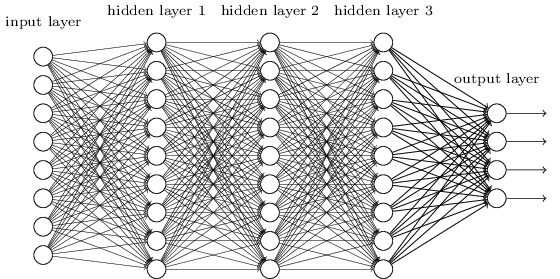
\includegraphics[width=0.7\textwidth]{img/dnn.png}
    \caption{Deep neural network}
    \label{fig:DNN}
\end{figure}

\subsubsection*{Monte Carlo Tree Search}

The neural network is trained from games of self-play by a reinforcement learning algorithm. In each position $s$, a Monte Carlo Tree Search is executed, guided by the neural network. The MCTS search outputs probabilities \(\pi\) of playing each move. These search probabilities usually select much stronger moves than the raw move probabilities $p$ of the neural network; MCTS may therefore be viewed as a powerful policy improvement operator. As shown in Figure \ref{fig:mcts}, this search algorithm consists to analyse the most promising moves, expanding the search tree based on random sampling of the search space. The application of Monte Carlo tree search in games is based on many playouts also called roll-outs. In each playout, the game is played out to the very end by selecting moves at random. The final game result of each playout is then used to weight the nodes in the game tree so that better nodes are more likely to be chosen in future playouts.

\begin{figure}[H]
    \centering
    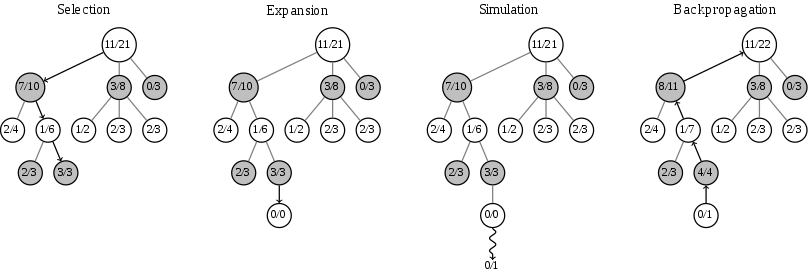
\includegraphics[width=0.7\textwidth]{img/mcts.png}
    \caption{Monte Carlo Tree Search}
    \label{fig:mcts}
\end{figure}

\subsubsection*{Simulations and results}

Although this algorithm is very powerful, it is strongly limited by the computation power available in the common machines. Indeed, training such a network has been very difficult due to the computation required to play each game. We thus received few samples of data, and these samples could not allow our agent to reach a top human player level.

The algorithm has been tested 100 times against the main previous agents. The results give 95\% of victory against the random agent, 55\% against the basic agent, and 25\% against the smart agent. Even if these results are not as good as expected, it is important to notice the very original method that we have used. It is thus still very convincing to see pretty good results with network that has never been trained by ourselves and without any evaluation function specific to this game.

%\bibliographystyle{srt}
\bibliography{bib.bib}

\end{document}
